\documentclass[11pt]{article}

\usepackage[margin=1in]{geometry}
\usepackage[T1]{fontenc}
\usepackage{graphicx}
\usepackage{longtable}
\usepackage{booktabs}
\usepackage{array}
\usepackage{enumitem}
\usepackage{xcolor}
\usepackage{hyperref}
\usepackage{tikz}
\usepackage{float}
\usepackage{fancyhdr}
\usepackage{titlesec}
\usepackage{tcolorbox}
\usepackage{tabularx}
\usepackage{multirow}
\usepackage{caption}
\usepackage{makecell}
\usepackage{amssymb}
\usepackage{pifont}

\usetikzlibrary{shapes.geometric, arrows.meta, positioning, fit, backgrounds, calc, decorations.pathreplacing, shapes.multipart, matrix, shadows}

% ---------------------------------------------------------------------------
% Color Definitions
% ---------------------------------------------------------------------------
\definecolor{sectionblue}{RGB}{31,78,121}
\definecolor{rupcolor}{RGB}{0,102,153}
\definecolor{vbcolor}{RGB}{60,179,113}
\definecolor{usecasecolor}{RGB}{255,193,7}
\definecolor{logicalcolor}{RGB}{70,130,180}
\definecolor{implcolor}{RGB}{40,167,69}
\definecolor{processcolor}{RGB}{220,53,69}
\definecolor{deploycolor}{RGB}{255,127,80}
\definecolor{flowcolor}{RGB}{100,100,100}
\definecolor{lightgray}{RGB}{245,245,245}
\definecolor{warningred}{RGB}{220,53,69}
\definecolor{successgreen}{RGB}{40,167,69}
\definecolor{infoblue}{RGB}{23,162,184}
\definecolor{phasecolor}{RGB}{128,0,128}
\definecolor{modulecolor}{RGB}{144,238,144}
\definecolor{cnccolor}{RGB}{255,182,193}
\definecolor{alloccolor}{RGB}{173,216,230}
\definecolor{umlcolor}{RGB}{255,218,185}

\hypersetup{
  colorlinks=true,
  linkcolor=sectionblue,
  urlcolor=sectionblue,
  citecolor=sectionblue
}

% ---------------------------------------------------------------------------
% Header and Footer
% ---------------------------------------------------------------------------
\pagestyle{fancy}
\fancyhf{}
\fancyhead[L]{\leftmark}
\fancyhead[R]{RUP / Views \& Beyond Integration}
\fancyfoot[C]{\thepage}
\renewcommand{\headrulewidth}{0.4pt}
\renewcommand{\footrulewidth}{0.4pt}

% ---------------------------------------------------------------------------
% Section Formatting
% ---------------------------------------------------------------------------
\titleformat{\section}
  {\normalfont\Large\bfseries\color{sectionblue}}{\thesection}{1em}{}
\titleformat{\subsection}
  {\normalfont\large\bfseries\color{sectionblue!80}}{\thesubsection}{1em}{}
\titleformat{\subsubsection}
  {\normalfont\normalsize\bfseries\color{sectionblue!60}}{\thesubsubsection}{1em}{}

% ---------------------------------------------------------------------------
% Custom Box Environments
% ---------------------------------------------------------------------------
\newtcolorbox{keypoint}{
    colback=blue!5,
    colframe=sectionblue,
    title=Key Point,
    fonttitle=\bfseries
}

\newtcolorbox{warning}{
    colback=red!5,
    colframe=warningred,
    title=Warning,
    fonttitle=\bfseries
}

\newtcolorbox{bestpractice}{
    colback=green!5,
    colframe=successgreen,
    title=Best Practice,
    fonttitle=\bfseries
}

\newtcolorbox{example}{
    colback=lightgray,
    colframe=flowcolor,
    title=Example,
    fonttitle=\bfseries
}

\newtcolorbox{definition}{
    colback=infoblue!10,
    colframe=infoblue,
    title=Definition,
    fonttitle=\bfseries
}

\newtcolorbox{rupbox}[1][]{
    colback=rupcolor!8,
    colframe=rupcolor,
    title=#1,
    fonttitle=\bfseries,
    breakable
}

\newtcolorbox{vbbox}[1][]{
    colback=vbcolor!10,
    colframe=vbcolor,
    title=#1,
    fonttitle=\bfseries,
    breakable
}

\newtcolorbox{mappingbox}[1][]{
    colback=usecasecolor!15,
    colframe=usecasecolor!80!black,
    title=#1,
    fonttitle=\bfseries
}

\newtcolorbox{phasebox}[1][]{
    colback=phasecolor!10,
    colframe=phasecolor,
    title=#1,
    fonttitle=\bfseries
}

\newtcolorbox{umlbox}[1][]{
    colback=umlcolor!30,
    colframe=umlcolor!70!black,
    title=#1,
    fonttitle=\bfseries
}

\newtcolorbox{checklistbox}[1][]{
    colback=white,
    colframe=flowcolor,
    title=#1,
    fonttitle=\bfseries
}

\tcbuselibrary{listings,breakable}

% ---------------------------------------------------------------------------
% List Settings
% ---------------------------------------------------------------------------
\setlist[itemize]{leftmargin=*,topsep=3pt,itemsep=2pt,parsep=0pt}
\setlist[enumerate]{leftmargin=*,topsep=3pt,itemsep=2pt,parsep=0pt}

% ---------------------------------------------------------------------------
% Custom Column Types
% ---------------------------------------------------------------------------
\newcolumntype{L}[1]{>{\raggedright\arraybackslash}p{#1}}
\newcolumntype{C}[1]{>{\centering\arraybackslash}p{#1}}
\newcolumntype{R}[1]{>{\raggedleft\arraybackslash}p{#1}}

% ---------------------------------------------------------------------------
% Custom Commands
% ---------------------------------------------------------------------------
\newcommand{\rup}{RUP}
\newcommand{\vb}{Views \& Beyond}
\newcommand{\usecaseview}{\textcolor{usecasecolor!80!black}{\textbf{Use Case}}}
\newcommand{\logicalview}{\textcolor{logicalcolor}{\textbf{Logical}}}
\newcommand{\implview}{\textcolor{implcolor}{\textbf{Implementation}}}
\newcommand{\processview}{\textcolor{processcolor}{\textbf{Process}}}
\newcommand{\deployview}{\textcolor{deploycolor}{\textbf{Deployment}}}

% ---------------------------------------------------------------------------
% Title
% ---------------------------------------------------------------------------
\title{%
    \vspace{-1cm}
    \textbf{\Huge Software Architecture Documentation}\\[12pt]
    \Large Integrating RUP 4+1 Views with Views and Beyond\\[8pt]
    \large A Comprehensive Guide to Mapping the Kruchten Model\\
    to SEI Documentation Practices
}
\author{%
    \textit{Architecture Documentation Series}\\[4pt]
    \small Based on Rational Unified Process and SEI Views and Beyond
}
\date{\today}

\begin{document}
\maketitle
\thispagestyle{empty}

\vspace{0.5cm}

\begin{abstract}
\noindent
The Rational Unified Process (RUP) and its underlying 4+1 View Model, introduced by Philippe Kruchten, has been one of the most influential approaches to software architecture organization. The SEI's Views and Beyond approach provides comprehensive guidance for documenting software architectures using a stakeholder-driven, view-based methodology. This guide provides detailed mappings between the five RUP architectural views (Use Case, Logical, Implementation, Process, and Deployment) and the Views and Beyond view types, covering UML diagram usage, RUP artifacts, phase-specific documentation needs, and practical guidance for creating documentation that satisfies both RUP practitioners and V\&B methodologists. Whether you are working in a RUP-based organization or transitioning to modern documentation practices, this guide provides the integration knowledge you need.
\end{abstract}

\vfill

\begin{center}
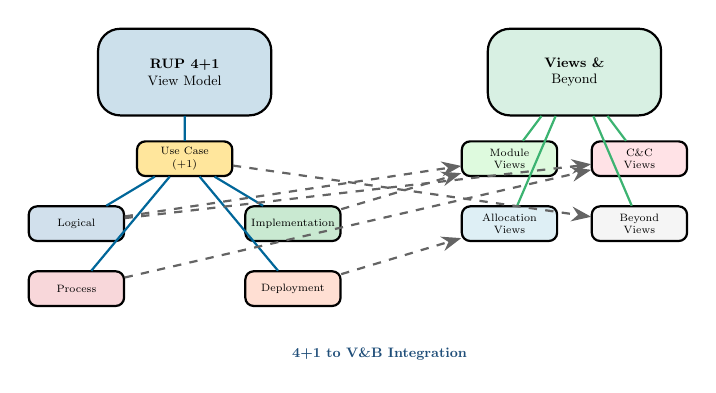
\begin{tikzpicture}[
    scale=0.55,
    transform shape,
    framework/.style={draw, thick, rounded corners=8pt, minimum width=4cm, minimum height=2cm, font=\small, align=center},
    viewpoint/.style={draw, thick, rounded corners=3pt, minimum width=2.2cm, minimum height=0.8cm, font=\scriptsize, align=center},
    arrow/.style={-{Stealth[length=2.5mm]}, thick, dashed}
]
    % RUP side (4+1)
    \node[framework, fill=rupcolor!20] (rup) at (-4.5,3.5) {\textbf{RUP 4+1}\\View Model};
    
    % +1 (Use Case) in center
    \node[viewpoint, fill=usecasecolor!40] (usecase) at (-4.5,1.5) {Use Case\\(+1)};
    
    % 4 views around
    \node[viewpoint, fill=logicalcolor!25] (logical) at (-7,0) {Logical};
    \node[viewpoint, fill=implcolor!25] (impl) at (-2,0) {Implementation};
    \node[viewpoint, fill=processcolor!20] (process) at (-7,-1.5) {Process};
    \node[viewpoint, fill=deploycolor!25] (deploy) at (-2,-1.5) {Deployment};
    
    % V&B side
    \node[framework, fill=vbcolor!20] (vb) at (4.5,3.5) {\textbf{Views \&}\\Beyond};
    \node[viewpoint, fill=modulecolor!30] (mod) at (3,1.5) {Module\\Views};
    \node[viewpoint, fill=cnccolor!40] (cnc) at (6,1.5) {C\&C\\Views};
    \node[viewpoint, fill=alloccolor!40] (alloc) at (3,0) {Allocation\\Views};
    \node[viewpoint, fill=lightgray] (beyond) at (6,0) {Beyond\\Views};
    
    % Connections from frameworks
    \draw[thick, rupcolor] (rup) -- (usecase);
    \draw[thick, rupcolor] (usecase) -- (logical);
    \draw[thick, rupcolor] (usecase) -- (impl);
    \draw[thick, rupcolor] (usecase) -- (process);
    \draw[thick, rupcolor] (usecase) -- (deploy);
    
    \draw[thick, vbcolor] (vb) -- (mod);
    \draw[thick, vbcolor] (vb) -- (cnc);
    \draw[thick, vbcolor] (vb) -- (alloc);
    \draw[thick, vbcolor] (vb) -- (beyond);
    
    % Mapping arrows
    \draw[arrow, flowcolor] (usecase) -- (beyond);
    \draw[arrow, flowcolor] (logical) -- (mod);
    \draw[arrow, flowcolor] (logical) -- (cnc);
    \draw[arrow, flowcolor] (impl) -- (mod);
    \draw[arrow, flowcolor] (process) -- (cnc);
    \draw[arrow, flowcolor] (deploy) -- (alloc);
    
    % Label
    \node[font=\bfseries\small, text=sectionblue] at (0,-3) {4+1 to V\&B Integration};
\end{tikzpicture}
\end{center}

\newpage
\tableofcontents
\newpage

%==============================================================================
\section{Introduction}
%==============================================================================

\subsection{Purpose of This Guide}

This guide provides comprehensive integration between the Rational Unified Process (RUP) 4+1 View Model and the SEI's Views and Beyond approach. Both frameworks are widely used, and practitioners often need to:

\begin{itemize}
    \item Translate RUP architectural artifacts to V\&B documentation
    \item Create documentation that satisfies stakeholders familiar with either approach
    \item Understand how UML diagrams map to V\&B view types
    \item Integrate RUP phase-based development with V\&B documentation practices
    \item Leverage the detailed guidance of V\&B within a RUP project
\end{itemize}

\subsection{The 4+1 View Model}

\begin{definition}
\textbf{4+1 View Model:} An architectural view model introduced by Philippe Kruchten in 1995, adopted by RUP. It organizes architecture description into four fundamental views (Logical, Implementation, Process, Deployment) plus one unifying view (Use Case) that ties the others together through scenarios.
\end{definition}

The ``+1'' (Use Case View) is central because it:
\begin{itemize}
    \item Provides scenarios that drive and validate the other four views
    \item Captures architecturally significant use cases
    \item Serves as input for test cases
    \item Represents stakeholder requirements
\end{itemize}

\begin{figure}[H]
\centering
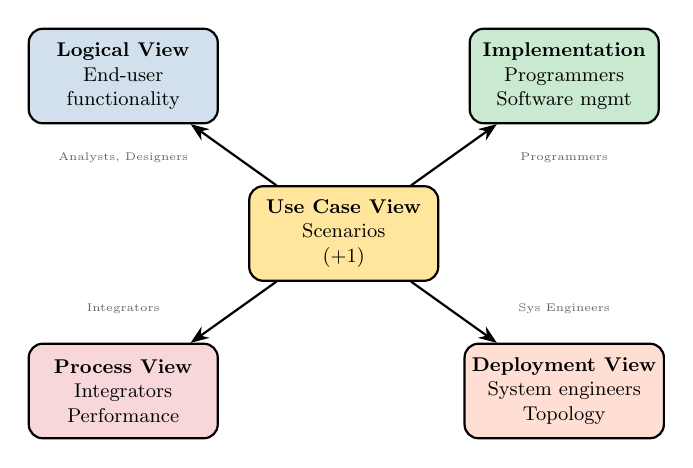
\begin{tikzpicture}[
    scale=0.8,
    transform shape,
    view/.style={draw, thick, fill=#1, minimum width=3cm, minimum height=1.5cm, rounded corners=5pt, font=\small, align=center}
]
    % Central Use Case view
    \node[view=usecasecolor!40] (uc) at (0,0) {\textbf{Use Case View}\\Scenarios\\(+1)};
    
    % Four surrounding views
    \node[view=logicalcolor!25] (log) at (-3.5,2.5) {\textbf{Logical View}\\End-user\\functionality};
    \node[view=implcolor!25] (impl) at (3.5,2.5) {\textbf{Implementation}\\Programmers\\Software mgmt};
    \node[view=processcolor!20] (proc) at (-3.5,-2.5) {\textbf{Process View}\\Integrators\\Performance};
    \node[view=deploycolor!25] (dep) at (3.5,-2.5) {\textbf{Deployment View}\\System engineers\\Topology};
    
    % Connections to center
    \draw[thick, -Stealth] (uc) -- (log);
    \draw[thick, -Stealth] (uc) -- (impl);
    \draw[thick, -Stealth] (uc) -- (proc);
    \draw[thick, -Stealth] (uc) -- (dep);
    
    % Labels for stakeholders
    \node[font=\tiny, text=flowcolor] at (-3.5,1.2) {Analysts, Designers};
    \node[font=\tiny, text=flowcolor] at (3.5,1.2) {Programmers};
    \node[font=\tiny, text=flowcolor] at (-3.5,-1.2) {Integrators};
    \node[font=\tiny, text=flowcolor] at (3.5,-1.2) {Sys Engineers};
\end{tikzpicture}
\caption{The 4+1 View Model}
\end{figure}

\subsection{Framework Comparison}

\begin{longtable}{@{}L{3cm} L{4.5cm} L{5cm}@{}}
\caption{Framework Comparison} \\
\toprule
\textbf{Aspect} & \textbf{RUP 4+1} & \textbf{Views and Beyond} \\
\midrule
\endfirsthead
\bottomrule
\endlastfoot
Origin & Rational Software (1995) & SEI Research (2002) \\
View Organization & 4+1 fixed views & 3 view categories + styles \\
Notation & UML-centric & Notation-agnostic \\
Scenarios & Central (+1 view) & Behavior documentation \\
Process Integration & RUP phases/iterations & Flexible integration \\
Documentation Unit & UML diagrams & View packets \\
Flexibility & Prescribed views & Stakeholder-driven selection \\
Quality Attributes & Implicit in views & Explicit scenarios/tactics \\
\end{longtable}

\subsection{Core Conceptual Mappings}

\begin{longtable}{@{}L{4cm} L{4cm} L{4.5cm}@{}}
\caption{Conceptual Term Mappings} \\
\toprule
\textbf{RUP Term} & \textbf{V\&B Term} & \textbf{Notes} \\
\midrule
\endfirsthead
\bottomrule
\endlastfoot
View & View & Work product showing structure \\
Use Case & Scenario / Behavior & Behavioral specification \\
Package & Module & Grouping of elements \\
Class & Module element & Code-time unit \\
Component & Component (C\&C) & Runtime unit \\
Node & Environment element & Physical resource \\
Artifact & Documentation unit & Work product \\
Subsystem & Module / Component & Context-dependent \\
\end{longtable}

%==============================================================================
\section{RUP Overview}
%==============================================================================

\subsection{RUP Phases and Architecture}

RUP defines four phases with architecture playing different roles in each:

\begin{figure}[H]
\centering
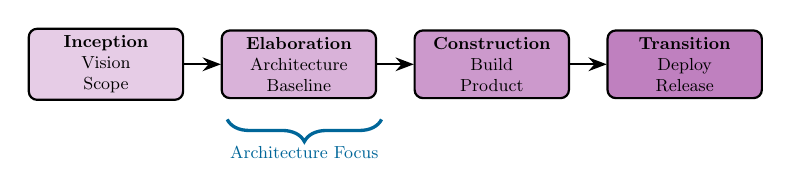
\begin{tikzpicture}[
    scale=0.7,
    transform shape,
    phase/.style={draw, thick, fill=#1, minimum width=2.8cm, minimum height=1.2cm, rounded corners=3pt, font=\small, align=center}
]
    % Phases
    \node[phase=phasecolor!20] (inc) at (0,0) {\textbf{Inception}\\Vision\\Scope};
    \node[phase=phasecolor!30] (elab) at (3.5,0) {\textbf{Elaboration}\\Architecture\\Baseline};
    \node[phase=phasecolor!40] (const) at (7,0) {\textbf{Construction}\\Build\\Product};
    \node[phase=phasecolor!50] (trans) at (10.5,0) {\textbf{Transition}\\Deploy\\Release};
    
    % Arrows
    \draw[thick, -Stealth] (inc) -- (elab);
    \draw[thick, -Stealth] (elab) -- (const);
    \draw[thick, -Stealth] (const) -- (trans);
    
    % Architecture emphasis line
    \draw[very thick, rupcolor, decorate, decoration={brace, amplitude=8pt, mirror}] 
        (2.2,-1) -- (5,-1) node[midway, below=10pt, font=\small, text=rupcolor] {Architecture Focus};
\end{tikzpicture}
\caption{RUP Phases and Architecture Focus}
\end{figure}

\begin{longtable}{@{}L{2.5cm} L{4cm} L{6cm}@{}}
\caption{Architecture Documentation by RUP Phase} \\
\toprule
\textbf{Phase} & \textbf{Architecture Focus} & \textbf{Documentation Needs} \\
\midrule
\endfirsthead
\bottomrule
\endlastfoot
Inception & Initial architecture vision & High-level views; Key use cases; Initial deployment concepts \\
Elaboration & Architecture baseline & Complete 4+1 views; Architectural mechanisms; Prototype validation \\
Construction & Architecture refinement & Detailed component specs; Interface documentation; Build procedures \\
Transition & Architecture validation & Deployment documentation; Operations support; Migration guides \\
\end{longtable}

\subsection{RUP Architectural Artifacts}

\begin{longtable}{@{}L{3.5cm} L{4cm} L{5cm}@{}}
\caption{RUP Architectural Artifacts} \\
\toprule
\textbf{Artifact} & \textbf{Description} & \textbf{V\&B Equivalent} \\
\midrule
\endfirsthead
\bottomrule
\endlastfoot
Software Architecture Document (SAD) & Main architecture description & Architecture documentation package \\
Use Case Model & Use case diagrams and specifications & Behavior documentation; Scenarios \\
Design Model & Class and interaction diagrams & Module views; C\&C views \\
Implementation Model & Component organization & Module decomposition view \\
Deployment Model & Node and artifact mapping & Deployment view \\
Data Model & Persistent data structure & Data model view \\
Analysis Model & Conceptual model & Context; High-level views \\
\end{longtable}

\subsection{UML Diagrams in RUP}

RUP relies heavily on UML for architectural representation:

\begin{longtable}{@{}L{3cm} L{3.5cm} L{3cm} L{3cm}@{}}
\caption{UML Diagrams by RUP View} \\
\toprule
\textbf{RUP View} & \textbf{Primary UML Diagrams} & \textbf{Secondary Diagrams} & \textbf{V\&B View Type} \\
\midrule
\endfirsthead
\bottomrule
\endlastfoot
Use Case & Use Case Diagram & Activity Diagram & Beyond Views \\
Logical & Class Diagram; Package Diagram & Object Diagram; Sequence Diagram & Module; C\&C \\
Implementation & Component Diagram; Package Diagram & Class Diagram & Module \\
Process & Activity Diagram; Sequence Diagram; State Machine & Communication Diagram & C\&C \\
Deployment & Deployment Diagram & Component Diagram & Allocation \\
\end{longtable}

%==============================================================================
\section{Use Case View Mapping}
%==============================================================================

\begin{rupbox}[RUP Use Case View]
\textbf{Purpose:} Contains architecturally significant use cases and scenarios that drive and validate the architecture. The ``+1'' that ties all other views together.

\textbf{Concerns Addressed:}
\begin{itemize}[nosep]
    \item System functionality from user perspective
    \item Architecturally significant requirements
    \item Scenario-based validation
    \item Stakeholder communication
\end{itemize}

\textbf{UML Diagrams:}
\begin{itemize}[nosep]
    \item Use Case Diagrams (actors, use cases, relationships)
    \item Activity Diagrams (workflow for complex use cases)
    \item Sequence Diagrams (scenario realizations)
\end{itemize}

\textbf{Stakeholders:} All stakeholders; particularly customers, users, analysts
\end{rupbox}

\begin{vbbox}[Views and Beyond Equivalent]
\textbf{Primary Mapping:} Documentation Beyond Views + Behavior Documentation

Use cases in V\&B are not a separate view but serve as:

\begin{itemize}
    \item \textbf{Behavior Documentation:} Use cases specify behavior and can be associated with any view where the behavior is realized
    \item \textbf{Quality Attribute Scenarios:} Architecturally significant use cases map to quality attribute scenarios
    \item \textbf{System Overview:} High-level use cases appear in documentation beyond views
    \item \textbf{View Rationale:} Use cases justify architectural decisions
\end{itemize}

\textbf{Key Insight:} V\&B treats scenarios/use cases as cross-cutting documentation that illuminates views rather than as a separate view type.
\end{vbbox}

\begin{mappingbox}[Implementation Mapping for Use Case View]

\textbf{RUP Use Case Diagram} $\rightarrow$ \textbf{V\&B Context + Behavior}
\begin{itemize}[nosep]
    \item Actors $\rightarrow$ External entities in context diagram
    \item Use cases $\rightarrow$ Behavior documentation; Quality scenarios
    \item System boundary $\rightarrow$ Context diagram boundary
\end{itemize}

\textbf{RUP Use Case Specifications} $\rightarrow$ \textbf{V\&B Behavior Documentation}
\begin{itemize}[nosep]
    \item Main flow $\rightarrow$ Behavior traces
    \item Alternative flows $\rightarrow$ Variability in behavior
    \item Pre/post conditions $\rightarrow$ Scenario constraints
\end{itemize}

\textbf{RUP Sequence Diagrams (Realizations)} $\rightarrow$ \textbf{V\&B View Behavior}
\begin{itemize}[nosep]
    \item Scenario realizations $\rightarrow$ Behavior documentation within C\&C view
    \item Component interactions $\rightarrow$ Sequence/trace notation
\end{itemize}

\textbf{Architecturally Significant Use Cases} $\rightarrow$ \textbf{V\&B Quality Attribute Scenarios}
\begin{itemize}[nosep]
    \item Performance-critical scenarios $\rightarrow$ Performance QA scenarios
    \item Security scenarios $\rightarrow$ Security QA scenarios
    \item Failure scenarios $\rightarrow$ Availability QA scenarios
\end{itemize}
\end{mappingbox}

\begin{example}
\textbf{Use Case to V\&B Mapping Example}

\textbf{RUP Architecturally Significant Use Case:}
\begin{quote}
UC-042: Process High-Volume Order Batch\\
Actor: Batch Scheduler\\
Precondition: Order queue contains 10,000+ orders\\
Main Flow: System processes all orders within 30 minutes maintaining data integrity\\
Quality: Performance-critical; Availability-critical
\end{quote}

\textbf{V\&B Documentation:}

\textit{Quality Attribute Scenario (Performance):}
\begin{itemize}[nosep]
    \item Source: Batch Scheduler
    \item Stimulus: 10,000 orders submitted
    \item Artifact: Order Processing System
    \item Environment: Normal batch window
    \item Response: Process all orders
    \item Measure: Complete within 30 minutes
\end{itemize}

\textit{C\&C View Behavior Documentation:}
Sequence diagram showing OrderProcessor, ValidationService, InventoryService, and FulfillmentService interactions during batch processing.

\textit{Rationale Reference:}
``Decision to use asynchronous processing with Kafka (ADR-007) directly supports UC-042 batch processing requirements.''
\end{example}

%==============================================================================
\section{Logical View Mapping}
%==============================================================================

\begin{rupbox}[RUP Logical View]
\textbf{Purpose:} Describes the system's key abstractions and mechanisms, primarily through classes, packages, and their relationships. Shows the logical organization that supports functionality.

\textbf{Concerns Addressed:}
\begin{itemize}[nosep]
    \item Functional requirements realization
    \item Key abstractions and their responsibilities
    \item Inheritance and composition relationships
    \item Package organization
    \item Design patterns and mechanisms
\end{itemize}

\textbf{UML Diagrams:}
\begin{itemize}[nosep]
    \item Class Diagrams (classes, interfaces, relationships)
    \item Package Diagrams (logical groupings)
    \item Object Diagrams (runtime instances)
    \item Interaction Diagrams (collaborations)
\end{itemize}

\textbf{Stakeholders:} Designers, developers, analysts
\end{rupbox}

\begin{vbbox}[Views and Beyond Equivalent]
\textbf{Primary Mapping:} Module Views (structural) + C\&C Views (runtime)

The Logical View maps to multiple V\&B view types:

\textbf{For Structural/Static Aspects:}
\begin{itemize}
    \item \textbf{Decomposition Style:} Package hierarchy and module organization
    \item \textbf{Generalization Style:} Inheritance relationships
    \item \textbf{Uses Style:} Dependencies between modules
    \item \textbf{Data Model Style:} Persistent class structures
\end{itemize}

\textbf{For Runtime/Dynamic Aspects:}
\begin{itemize}
    \item \textbf{Client-Server C\&C:} Request-response interactions
    \item \textbf{Object-Oriented C\&C:} Object collaborations
    \item \textbf{Shared-Data C\&C:} Repository interactions
\end{itemize}

\textbf{Key Insight:} RUP's Logical View conflates code-time structure (Module) with runtime behavior (C\&C). V\&B separates these concerns.
\end{vbbox}

\begin{mappingbox}[Implementation Mapping for Logical View]

\textbf{RUP Class Diagram (Structure)} $\rightarrow$ \textbf{V\&B Module Views}
\begin{itemize}[nosep]
    \item Classes $\rightarrow$ Modules in decomposition
    \item Interfaces $\rightarrow$ Module interfaces
    \item Inheritance $\rightarrow$ Generalization view (is-a relations)
    \item Dependencies $\rightarrow$ Uses view (allowed-to-use relations)
    \item Associations $\rightarrow$ Module relations in element catalog
\end{itemize}

\textbf{RUP Package Diagram} $\rightarrow$ \textbf{V\&B Decomposition View}
\begin{itemize}[nosep]
    \item Packages $\rightarrow$ Modules (parent modules)
    \item Package dependencies $\rightarrow$ Uses relations
    \item Package hierarchy $\rightarrow$ Decomposition hierarchy
\end{itemize}

\textbf{RUP Interaction Diagrams} $\rightarrow$ \textbf{V\&B C\&C View + Behavior}
\begin{itemize}[nosep]
    \item Objects $\rightarrow$ Component instances
    \item Messages $\rightarrow$ Connector interactions
    \item Sequence $\rightarrow$ Behavior documentation (traces)
\end{itemize}

\textbf{RUP Design Patterns/Mechanisms} $\rightarrow$ \textbf{V\&B Rationale}
\begin{itemize}[nosep]
    \item Architectural mechanisms $\rightarrow$ Documented in rationale
    \item Pattern applications $\rightarrow$ Decision records
\end{itemize}
\end{mappingbox}

\begin{warning}
\textbf{Common Mapping Pitfall}

RUP's Logical View often mixes static class structure with dynamic object interactions in a single view. When mapping to V\&B:

\begin{enumerate}
    \item \textbf{Separate structural from behavioral:} Class relationships go in Module views; object interactions go in C\&C views with behavior documentation
    \item \textbf{Distinguish compile-time from runtime:} Class diagrams showing code structure are Module; diagrams showing runtime objects are C\&C
    \item \textbf{Be explicit about instances:} If showing specific runtime instances, use C\&C; if showing types/classes, use Module
\end{enumerate}
\end{warning}

%==============================================================================
\section{Implementation View Mapping}
%==============================================================================

\begin{rupbox}[RUP Implementation View]
\textbf{Purpose:} Describes the organization of static software elements (code, data, components) in the development environment. Shows how design elements map to implementation artifacts.

\textbf{Concerns Addressed:}
\begin{itemize}[nosep]
    \item Source code organization
    \item Component packaging
    \item Build dependencies
    \item Configuration management
    \item Layer organization
\end{itemize}

\textbf{UML Diagrams:}
\begin{itemize}[nosep]
    \item Component Diagrams (software components)
    \item Package Diagrams (source organization)
    \item Class Diagrams (implementation classes)
\end{itemize}

\textbf{Stakeholders:} Programmers, software managers, build engineers
\end{rupbox}

\begin{vbbox}[Views and Beyond Equivalent]
\textbf{Primary Mapping:} Module Views + Implementation Allocation View

\begin{itemize}
    \item \textbf{Decomposition Style:} Module hierarchy showing component organization
    \item \textbf{Layered Style:} Layer structure with allowed dependencies
    \item \textbf{Uses Style:} Build-time dependencies
    \item \textbf{Implementation View (Allocation):} Mapping to source files and directories
\end{itemize}

\textbf{Key Distinction:} RUP's ``Implementation View'' focuses on component packaging. V\&B's ``Implementation View'' (allocation style) specifically maps modules to file system. Both address developer concerns but with different scope.
\end{vbbox}

\begin{mappingbox}[Implementation Mapping for Implementation View]

\textbf{RUP Component Diagram} $\rightarrow$ \textbf{V\&B Module Views}
\begin{itemize}[nosep]
    \item Components $\rightarrow$ Modules in decomposition
    \item Component interfaces $\rightarrow$ Module interfaces
    \item Component dependencies $\rightarrow$ Uses relations
    \item Provided/Required interfaces $\rightarrow$ Interface documentation
\end{itemize}

\textbf{RUP Source Organization} $\rightarrow$ \textbf{V\&B Implementation View (Allocation)}
\begin{itemize}[nosep]
    \item Source directories $\rightarrow$ File system structure
    \item Module-to-file mapping $\rightarrow$ Implementation allocation
    \item Build artifacts $\rightarrow$ Build output mapping
\end{itemize}

\textbf{RUP Layer Structure} $\rightarrow$ \textbf{V\&B Layered View}
\begin{itemize}[nosep]
    \item Layers $\rightarrow$ Layers in layered view
    \item Layer rules $\rightarrow$ Allowed-to-use constraints
    \item Layer contents $\rightarrow$ Layer decomposition
\end{itemize}

\textbf{RUP Subsystems} $\rightarrow$ \textbf{V\&B Module Decomposition}
\begin{itemize}[nosep]
    \item Subsystems $\rightarrow$ Top-level modules
    \item Subsystem interfaces $\rightarrow$ Module public interfaces
    \item Internal components $\rightarrow$ Child modules
\end{itemize}
\end{mappingbox}

\begin{example}
\textbf{Implementation View Mapping Example}

\textbf{RUP Component Diagram:}
\begin{verbatim}
<<component>> OrderManagement
  - provides: IOrderService
  - requires: IInventory, IPayment
  - contains: OrderValidator, OrderProcessor, OrderRepository
\end{verbatim}

\textbf{V\&B Module Decomposition:}

\textit{Element Catalog Entry:}

\textbf{Module:} OrderManagement

\textbf{Responsibilities:} Order lifecycle management; validation; persistence

\textbf{Interfaces:}
\begin{itemize}[nosep]
    \item IOrderService (provided): Order CRUD operations
\end{itemize}

\textbf{Children:}
\begin{itemize}[nosep]
    \item OrderValidator: Input validation logic
    \item OrderProcessor: Business logic orchestration
    \item OrderRepository: Data access layer
\end{itemize}

\textbf{Uses Relations:}
\begin{itemize}[nosep]
    \item Uses InventoryManagement.IInventory
    \item Uses PaymentProcessing.IPayment
\end{itemize}

\textbf{V\&B Implementation View (Allocation):}
\begin{verbatim}
OrderManagement -> /src/main/java/com/acme/orders/
  OrderValidator -> OrderValidator.java
  OrderProcessor -> OrderProcessor.java
  OrderRepository -> OrderRepository.java
  IOrderService -> interfaces/IOrderService.java
\end{verbatim}
\end{example}

%==============================================================================
\section{Process View Mapping}
%==============================================================================

\begin{rupbox}[RUP Process View]
\textbf{Purpose:} Describes the system's concurrency and synchronization aspects. Shows processes, threads, and their interactions to address performance, scalability, and throughput.

\textbf{Concerns Addressed:}
\begin{itemize}[nosep]
    \item Concurrency and parallelism
    \item Process/thread structure
    \item Synchronization and locking
    \item Inter-process communication
    \item Performance and scalability
    \item Fault tolerance
\end{itemize}

\textbf{UML Diagrams:}
\begin{itemize}[nosep]
    \item Activity Diagrams (parallel flows, synchronization)
    \item Sequence Diagrams (process interactions)
    \item State Machine Diagrams (process states)
    \item Communication Diagrams (process topology)
\end{itemize}

\textbf{Stakeholders:} System integrators, performance engineers, developers
\end{rupbox}

\begin{vbbox}[Views and Beyond Equivalent]
\textbf{Primary Mapping:} Communicating-Processes C\&C Style

\begin{itemize}
    \item \textbf{Communicating-Processes Style:} Primary style for process/thread structure
    \item \textbf{Pipe-and-Filter Style:} For data processing pipelines
    \item \textbf{Shared-Data Style:} For shared memory communication
    \item \textbf{Client-Server Style:} For request-handling processes
\end{itemize}

\textbf{C\&C View Elements:}
\begin{itemize}
    \item Components: Processes, threads, tasks
    \item Connectors: IPC mechanisms, synchronization primitives, message queues
    \item Properties: Thread safety, concurrency constraints, scheduling
\end{itemize}

\textbf{Behavior Documentation:} State machines and interaction traces document process behavior.
\end{vbbox}

\begin{mappingbox}[Implementation Mapping for Process View]

\textbf{RUP Process Structure} $\rightarrow$ \textbf{V\&B C\&C Communicating-Processes}
\begin{itemize}[nosep]
    \item Processes $\rightarrow$ Process components
    \item Threads $\rightarrow$ Thread components (or component properties)
    \item Process groups $\rightarrow$ Component groupings
\end{itemize}

\textbf{RUP IPC Mechanisms} $\rightarrow$ \textbf{V\&B Connectors}
\begin{itemize}[nosep]
    \item Message passing $\rightarrow$ Message connector type
    \item Shared memory $\rightarrow$ Shared-data connector
    \item RPC/RMI $\rightarrow$ Call-return connector
    \item Events/Signals $\rightarrow$ Event connector
\end{itemize}

\textbf{RUP Synchronization} $\rightarrow$ \textbf{V\&B Connector Properties}
\begin{itemize}[nosep]
    \item Locks/Mutexes $\rightarrow$ Synchronization properties
    \item Semaphores $\rightarrow$ Concurrency constraints
    \item Barriers $\rightarrow$ Synchronization points
\end{itemize}

\textbf{RUP Activity Diagrams (Concurrent)} $\rightarrow$ \textbf{V\&B Behavior Documentation}
\begin{itemize}[nosep]
    \item Parallel flows $\rightarrow$ Concurrent trace notation
    \item Join/Fork $\rightarrow$ Synchronization in behavior
    \item Swimlanes $\rightarrow$ Process allocation
\end{itemize}

\textbf{RUP State Machines} $\rightarrow$ \textbf{V\&B Behavior Documentation}
\begin{itemize}[nosep]
    \item Process states $\rightarrow$ State diagrams in C\&C view
    \item State transitions $\rightarrow$ State machine notation
\end{itemize}
\end{mappingbox}

%==============================================================================
\section{Deployment View Mapping}
%==============================================================================

\begin{rupbox}[RUP Deployment View]
\textbf{Purpose:} Describes the mapping of software to hardware, showing nodes, their connections, and the software artifacts deployed on each node.

\textbf{Concerns Addressed:}
\begin{itemize}[nosep]
    \item Hardware topology
    \item Software-to-hardware mapping
    \item Network configuration
    \item Distribution and communication
    \item System installation
\end{itemize}

\textbf{UML Diagrams:}
\begin{itemize}[nosep]
    \item Deployment Diagrams (nodes, artifacts, connections)
    \item Component Diagrams (deployed components)
\end{itemize}

\textbf{Stakeholders:} System engineers, operators, network administrators
\end{rupbox}

\begin{vbbox}[Views and Beyond Equivalent]
\textbf{Primary Mapping:} Deployment Style (Allocation Views)

\begin{itemize}
    \item \textbf{Deployment View:} Primary allocation view for hardware mapping
    \item \textbf{Install View:} For installation structure (complements deployment)
\end{itemize}

\textbf{Deployment View Elements:}
\begin{itemize}
    \item Software elements: Components from C\&C views
    \item Environmental elements: Servers, containers, VMs, network zones
    \item Allocation relation: ``Deployed-on'' mapping
\end{itemize}

The V\&B Deployment view closely matches RUP's Deployment view, making this one of the most direct mappings.
\end{vbbox}

\begin{mappingbox}[Implementation Mapping for Deployment View]

\textbf{RUP Deployment Diagram} $\rightarrow$ \textbf{V\&B Deployment View}
\begin{itemize}[nosep]
    \item Nodes $\rightarrow$ Environmental elements (hosts)
    \item Artifacts $\rightarrow$ Software elements
    \item Deployed artifacts $\rightarrow$ Allocation relations
    \item Communication paths $\rightarrow$ Network connections
\end{itemize}

\textbf{RUP Node Properties} $\rightarrow$ \textbf{V\&B Element Catalog}
\begin{itemize}[nosep]
    \item Hardware specs $\rightarrow$ Node properties
    \item OS/middleware $\rightarrow$ Environment properties
    \item Capacity $\rightarrow$ Resource properties
\end{itemize}

\textbf{RUP Network Topology} $\rightarrow$ \textbf{V\&B Deployment View}
\begin{itemize}[nosep]
    \item Network connections $\rightarrow$ Communication paths
    \item Protocols $\rightarrow$ Connection properties
    \item Network zones $\rightarrow$ Environmental regions
\end{itemize}

\textbf{RUP Artifacts} $\rightarrow$ \textbf{V\&B Software Elements}
\begin{itemize}[nosep]
    \item Executables $\rightarrow$ Deployable units
    \item Libraries $\rightarrow$ Shared components
    \item Configuration files $\rightarrow$ Configuration elements
\end{itemize}
\end{mappingbox}

\begin{example}
\textbf{Deployment View Mapping Example}

\textbf{RUP Deployment Diagram:}
\begin{verbatim}
<<device>> WebServer
  <<artifact>> webapp.war
  <<artifact>> nginx.conf

<<device>> AppServer [3 instances]
  <<artifact>> orderservice.jar
  <<artifact>> inventoryservice.jar
  
<<device>> DatabaseServer
  <<artifact>> postgresql
  
WebServer --HTTP--> AppServer --JDBC--> DatabaseServer
\end{verbatim}

\textbf{V\&B Deployment View Element Catalog:}

\textbf{Environmental Elements:}
\begin{itemize}[nosep]
    \item \textbf{WebServer:} Nginx reverse proxy; 4 CPU, 8GB RAM; DMZ zone
    \item \textbf{AppServer:} Java application server; 8 CPU, 32GB RAM; Application zone; 3 instances for HA
    \item \textbf{DatabaseServer:} PostgreSQL 15; 16 CPU, 128GB RAM; Data zone; Primary + standby
\end{itemize}

\textbf{Allocation Relations:}
\begin{itemize}[nosep]
    \item WebServer hosts: webapp.war (frontend), nginx.conf (routing rules)
    \item AppServer hosts: OrderService, InventoryService, PaymentService
    \item DatabaseServer hosts: PostgreSQL (orders, inventory, payments schemas)
\end{itemize}

\textbf{Communication Paths:}
\begin{itemize}[nosep]
    \item WebServer $\rightarrow$ AppServer: HTTPS/443, load-balanced round-robin
    \item AppServer $\rightarrow$ DatabaseServer: JDBC/5432, connection pooled (max 50)
\end{itemize}
\end{example}

%==============================================================================
\section{UML Notation Mapping}
%==============================================================================

\subsection{UML Diagrams to V\&B View Types}

\begin{longtable}{@{}L{3cm} L{2.5cm} L{3cm} L{4cm}@{}}
\caption{UML Diagram to V\&B View Type Mapping} \\
\toprule
\textbf{UML Diagram} & \textbf{RUP View} & \textbf{V\&B View Type} & \textbf{Usage Notes} \\
\midrule
\endfirsthead
\toprule
\textbf{UML Diagram} & \textbf{RUP View} & \textbf{V\&B View Type} & \textbf{Usage Notes} \\
\midrule
\endhead
\bottomrule
\endlastfoot
Use Case Diagram & Use Case & Beyond Views; Context & System boundary; actors \\
Class Diagram & Logical & Module Views & Static structure \\
Package Diagram & Logical; Impl & Module Decomposition & Module hierarchy \\
Object Diagram & Logical & C\&C View & Runtime instances \\
Sequence Diagram & Use Case; Logical; Process & Behavior Documentation & Interaction traces \\
Communication Diagram & Logical; Process & C\&C + Behavior & Object/process topology \\
Activity Diagram & Use Case; Process & Behavior Documentation & Workflows; concurrency \\
State Machine & Logical; Process & Behavior Documentation & Element states \\
Component Diagram & Implementation & Module Views & Component organization \\
Deployment Diagram & Deployment & Deployment View (Allocation) & Hardware mapping \\
Composite Structure & Logical & C\&C View & Internal structure \\
\end{longtable}

\subsection{Notation Considerations}

\begin{umlbox}[UML in V\&B Documentation]
V\&B is notation-agnostic, but UML is a natural fit. When using UML:

\textbf{For Module Views:}
\begin{itemize}[nosep]
    \item Use Class Diagrams with ``is-part-of'' for decomposition
    \item Use Class Diagrams with generalization for generalization view
    \item Use Package Diagrams for high-level decomposition
    \item Annotate with \texttt{<<module>>} stereotype if needed
\end{itemize}

\textbf{For C\&C Views:}
\begin{itemize}[nosep]
    \item Use Component Diagrams with \texttt{<<component>>} stereotype
    \item Use Composite Structure for internal C\&C
    \item Clearly distinguish components from modules
    \item Show ports and connectors explicitly
\end{itemize}

\textbf{For Allocation Views:}
\begin{itemize}[nosep]
    \item Use Deployment Diagrams directly
    \item Show artifacts deployed on nodes
    \item Include communication paths with protocols
\end{itemize}

\textbf{For Behavior:}
\begin{itemize}[nosep]
    \item Use Sequence Diagrams for traces
    \item Use State Machines for stateful components
    \item Use Activity Diagrams for workflows
\end{itemize}
\end{umlbox}

%==============================================================================
\section{Complete Mapping Reference}
%==============================================================================

\begin{longtable}{@{}L{3cm} L{4.5cm} L{5cm}@{}}
\caption{Complete RUP to V\&B Mapping Reference} \\
\toprule
\textbf{RUP Element} & \textbf{V\&B Equivalent} & \textbf{Implementation Notes} \\
\midrule
\endfirsthead
\toprule
\textbf{RUP Element} & \textbf{V\&B Equivalent} & \textbf{Implementation Notes} \\
\midrule
\endhead
\bottomrule
\endlastfoot

\multicolumn{3}{l}{\textbf{Use Case View (+1)}} \\
\quad Use cases & Behavior documentation & Associate with views \\
\quad Actors & Context diagram entities & External actors \\
\quad Scenarios & Quality attribute scenarios & Architecturally significant \\
\quad Realizations & Behavior traces & In C\&C views \\
\midrule

\multicolumn{3}{l}{\textbf{Logical View}} \\
\quad Classes (structural) & Module decomposition & Code-time structure \\
\quad Classes (runtime) & C\&C components & Runtime instances \\
\quad Packages & Module hierarchy & Decomposition view \\
\quad Inheritance & Generalization view & Is-a relations \\
\quad Associations & Module relations & Element catalog \\
\quad Interactions & C\&C behavior & Sequence/trace \\
\quad Patterns & Rationale & Decision documentation \\
\midrule

\multicolumn{3}{l}{\textbf{Implementation View}} \\
\quad Components & Modules & Decomposition view \\
\quad Layers & Layered view & With constraints \\
\quad Source structure & Implementation view & Allocation style \\
\quad Dependencies & Uses view & Allowed-to-use \\
\quad Subsystems & Top-level modules & With interfaces \\
\midrule

\multicolumn{3}{l}{\textbf{Process View}} \\
\quad Processes & C\&C components & Communicating-processes \\
\quad Threads & Component properties & Or sub-components \\
\quad IPC & Connectors & Typed connectors \\
\quad Synchronization & Connector properties & Concurrency constraints \\
\quad Process states & Behavior documentation & State machines \\
\midrule

\multicolumn{3}{l}{\textbf{Deployment View}} \\
\quad Nodes & Environmental elements & Deployment view \\
\quad Artifacts & Software elements & Deployable units \\
\quad Deployment & Allocation relations & Deployed-on \\
\quad Network & Communication paths & With properties \\

\end{longtable}

%==============================================================================
\section{Implementation Guidance}
%==============================================================================

\subsection{Mapping Strategy}

\begin{bestpractice}
\textbf{RUP to V\&B Migration Strategy:}

\begin{enumerate}
    \item \textbf{Inventory existing artifacts:} List all RUP architectural artifacts (SAD sections, UML models)
    
    \item \textbf{Map to V\&B views:} Use this guide to identify V\&B view types for each RUP artifact
    
    \item \textbf{Separate concerns:} Split RUP Logical View into Module (structural) and C\&C (runtime) views
    
    \item \textbf{Extract behavior:} Move use case realizations and scenarios to behavior documentation
    
    \item \textbf{Add V\&B structure:} Create element catalogs, rationale, and variability guides
    
    \item \textbf{Create view packets:} Package views with all V\&B documentation components
\end{enumerate}
\end{bestpractice}

\subsection{Documentation Structure}

\begin{longtable}{@{}L{3cm} L{4.5cm} L{5cm}@{}}
\caption{RUP SAD Section to V\&B Mapping} \\
\toprule
\textbf{RUP SAD Section} & \textbf{V\&B Equivalent} & \textbf{Notes} \\
\midrule
\endfirsthead
\bottomrule
\endlastfoot
Introduction & Documentation Roadmap & Purpose, scope, definitions \\
Architectural Goals & Rationale; Quality Scenarios & Driving requirements \\
Use Case View & Beyond Views; Behavior & Cross-cutting scenarios \\
Logical View & Module Views; C\&C Views & Split static/dynamic \\
Implementation View & Module Views; Allocation & Code organization \\
Process View & C\&C Views & Concurrency structure \\
Deployment View & Allocation Views & Hardware mapping \\
Size and Performance & Quality Scenarios; Element Properties & Quantified requirements \\
Quality & Quality Scenarios; Rationale & Quality decisions \\
\end{longtable}

\subsection{Phase-Specific Documentation}

\begin{phasebox}[Documentation by RUP Phase]
\textbf{Inception Phase:}
\begin{itemize}[nosep]
    \item V\&B: System overview; Initial context diagram; Key quality scenarios
    \item Focus: Stakeholder identification; Architectural vision
\end{itemize}

\textbf{Elaboration Phase:}
\begin{itemize}[nosep]
    \item V\&B: Complete view packets for primary views; Element catalogs; Rationale
    \item Focus: Architecture baseline; Risk mitigation; View selection
\end{itemize}

\textbf{Construction Phase:}
\begin{itemize}[nosep]
    \item V\&B: Detailed element catalogs; Interface documentation; Behavior traces
    \item Focus: Implementation guidance; Integration support
\end{itemize}

\textbf{Transition Phase:}
\begin{itemize}[nosep]
    \item V\&B: Deployment views; Install views; Operational documentation
    \item Focus: Deployment support; Operations handoff
\end{itemize}
\end{phasebox}

\subsection{View Packet Completeness}

\begin{checklistbox}[V\&B View Packet Checklist (from RUP artifacts)]
\textbf{Primary Presentation:}
\begin{itemize}[leftmargin=1.5cm]
    \item[$\square$] UML diagram(s) from RUP view
    \item[$\square$] Notation key (if non-standard UML)
    \item[$\square$] Diagram purpose statement
\end{itemize}

\textbf{Element Catalog:}
\begin{itemize}[leftmargin=1.5cm]
    \item[$\square$] All elements from UML diagrams documented
    \item[$\square$] Element responsibilities (from class/component descriptions)
    \item[$\square$] Element interfaces
    \item[$\square$] Element properties (quality attributes)
    \item[$\square$] Relations documented
\end{itemize}

\textbf{Context Diagram:}
\begin{itemize}[leftmargin=1.5cm]
    \item[$\square$] System boundary (from Use Case diagram)
    \item[$\square$] External actors/systems
    \item[$\square$] External interfaces
\end{itemize}

\textbf{Behavior Documentation:}
\begin{itemize}[leftmargin=1.5cm]
    \item[$\square$] Use case realizations migrated
    \item[$\square$] Sequence diagrams included
    \item[$\square$] State machines for stateful elements
\end{itemize}

\textbf{Rationale:}
\begin{itemize}[leftmargin=1.5cm]
    \item[$\square$] Design decisions documented
    \item[$\square$] Pattern/mechanism justification
    \item[$\square$] Alternative analysis
\end{itemize}

\textbf{Variability Guide:}
\begin{itemize}[leftmargin=1.5cm]
    \item[$\square$] Variation points identified
    \item[$\square$] Configuration options
\end{itemize}
\end{checklistbox}

%==============================================================================
\section{Appendix A: Quick Reference Table}
%==============================================================================

\begin{longtable}{@{}L{4cm} L{8.5cm}@{}}
\caption{Quick Reference: RUP to V\&B} \\
\toprule
\textbf{RUP View} & \textbf{V\&B Approach} \\
\midrule
\endfirsthead
\bottomrule
\endlastfoot
Use Case View & Behavior documentation associated with views; Quality attribute scenarios in rationale; Context diagram for system boundary \\
\addlinespace[0.5em]
Logical View & Module views (Decomposition, Generalization, Uses) for structural aspects; C\&C views for runtime aspects \\
\addlinespace[0.5em]
Implementation View & Module views (Decomposition, Layered) for component structure; Implementation allocation view for source mapping \\
\addlinespace[0.5em]
Process View & C\&C Communicating-Processes style for concurrency; Behavior documentation for state and interaction \\
\addlinespace[0.5em]
Deployment View & Deployment allocation view; Install view for installation structure \\
\end{longtable}

%==============================================================================
\section{Appendix B: RUP Artifact Cross-Reference}
%==============================================================================

\begin{longtable}{@{}L{4cm} L{4cm} L{4.5cm}@{}}
\caption{RUP Artifacts to V\&B Documentation} \\
\toprule
\textbf{RUP Artifact} & \textbf{V\&B Documentation} & \textbf{Notes} \\
\midrule
\endfirsthead
\bottomrule
\endlastfoot
Software Architecture Document & Architecture Documentation Package & Complete view set \\
Use Case Model & Context + Behavior & System boundary; scenarios \\
Analysis Model & System Overview & High-level concepts \\
Design Model & Module + C\&C Views & Detailed structure \\
Data Model & Data Model View & Persistent data \\
Implementation Model & Decomposition + Implementation & Code structure \\
Deployment Model & Deployment View & Hardware mapping \\
Architectural Prototype & Rationale & Validation evidence \\
Reference Architecture & Documentation Beyond Views & Reusable patterns \\
Design Guidelines & Rationale; Beyond Views & Conventions \\
\end{longtable}

%==============================================================================
\section{Appendix C: Glossary}
%==============================================================================

\begin{description}[leftmargin=3cm, style=nextline]
    \item[4+1 View Model] Kruchten's architectural view organization with four views plus scenarios
    \item[Artifact] RUP term for a work product
    \item[C\&C View] Component-and-Connector view showing runtime structure
    \item[Component] Runtime unit with defined interfaces
    \item[Element Catalog] V\&B detailed element specifications
    \item[Module] Code-time unit (class, package, library)
    \item[Module View] V\&B view showing code-time structure
    \item[Process] Concurrent execution unit
    \item[RUP] Rational Unified Process
    \item[SAD] Software Architecture Document
    \item[Scenario] Use case or quality attribute scenario
    \item[Subsystem] RUP grouping of related components
    \item[View Packet] V\&B unit of view documentation
\end{description}

%==============================================================================
\section{Appendix D: References}
%==============================================================================

\begin{enumerate}
    \item Kruchten, P. (1995). ``The 4+1 View Model of Architecture.'' \textit{IEEE Software}, 12(6), 42-50.
    
    \item Kruchten, P. (2003). \textit{The Rational Unified Process: An Introduction} (3rd ed.). Addison-Wesley.
    
    \item Clements, P., et al. (2010). \textit{Documenting Software Architectures: Views and Beyond} (2nd ed.). Addison-Wesley.
    
    \item Bass, L., Clements, P., \& Kazman, R. (2021). \textit{Software Architecture in Practice} (4th ed.). Addison-Wesley.
    
    \item Rumbaugh, J., Jacobson, I., \& Booch, G. (2004). \textit{The Unified Modeling Language Reference Manual} (2nd ed.). Addison-Wesley.
    
    \item ISO/IEC/IEEE 42010:2011. \textit{Systems and software engineering---Architecture description}.
    
    \item Jacobson, I., Booch, G., \& Rumbaugh, J. (1999). \textit{The Unified Software Development Process}. Addison-Wesley.
    
    \item IBM Rational. (2006). \textit{Rational Unified Process: Best Practices for Software Development Teams}. IBM White Paper.
\end{enumerate}

\end{document}
